
\section{Scaling Options}

There are a various options which control or change the scaling of an axis.
Here, ``scaling'' typically means two aspects: first, the unit vector size in
each direction and second, the displayed limits in each direction. Both
together control the size of the axis box. In addition, axis descriptions
change the size. However, \PGFPlots{} scales only units and determines limits.
It does not scale axis descriptions by default in order to keep consistent font
sizes between the text and the figure.

Often, one wishes to provide the target size only and let \PGFPlots{} do the
rest. This is the default; it scales the axis to |width| and |height|. If you
provide one of these options, the axis will be rescaled while keeping the
aspect ratio.

Occasionally, one wants to provide unit vectors explicitly to ensure that one
unit takes a prescribed amount of space. This is possible by means of the |x|,
|y|, and |z| keys. In such a case, the |width| and |height| options will be
ignored (or only applied for the unspecified unit vectors).

Another common approach is to enforce specific |unit vector ratio|s: for
example by specifying that each unit should take the same amount of space using
|axis equal|. Here, \PGFPlots{} scales the lengths of all vectors uniformly,
i.e.\@ it applies the same scale to each vector. This is done by means of the
|scale mode| configuration which is basically one of
|scale mode=stretch to fill| or |scale mode=scale uniformly|: \PGFPlots{} tries
to satisfy the prescribed |width| and |height| arguments by finding a
\emph{common} scaling factor. In addition, it attempts to enlarge the limits
individually to fit into the prescribed dimensions.

In addition, you can use the option |/pgfplots/scale| to simply scale all final
units up by some prescribed factor. This does not change text labels.

If needed, you can also supply |/tikz/scale| to an axis. This will scale the
complete resulting image, including all text labels.


\subsection{Common Scaling Options}

All common options mentioned in the previous paragraphs are described here.

\begin{pgfplotskey}{width=\marg{dimen} (initially empty)}
    Sets the width of the final picture to \marg{dimen}.

    Any non-empty dimension like |width=5cm| sets the desired target width. Any
    \TeX{} unit is accepted (like |200pt| or |5in|).

    An empty value |width={}| means ``use default width or rescale
    proportionally to |height|''. In this case, \PGFPlots{} uses the value of
    |\axisdefaultwidth| as target quantity. However, if the |height| key has
    been set, \PGFPlots{} will rescale the |\axisdefaultwidth| in a way which
    keeps the ratio between |\axisdefaultwidth| and |\axisdefaultheight|. This
    allows to specify just one of |width| and |height| and keep aspect ratios.

    Consequently, if you specify just |width=5cm| but leave the default
    |height={}|, the scaling will respect the initial aspect ratio.

    The scaling affects the unit vectors for $x$, $y$, and $z$. It does not
    change the size of text labels or axis descriptions.
    %
\begin{codeexample}[]
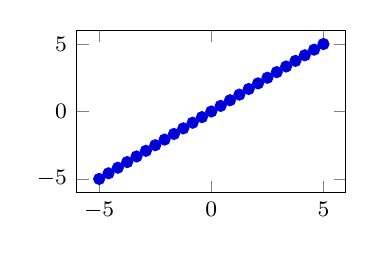
\begin{tikzpicture}
\begin{axis}[
    width=5cm,
]
    \addplot {x};
\end{axis}
\end{tikzpicture}
\end{codeexample}

    Please note that \PGFPlots{} only estimates the size needed for axis- and
    tick labels. The estimate assumes a fixed amount of space for anything
    which is outside of the axis box. This has the effect that the final images
    may be slightly larger or slightly smaller than the prescribed dimensions.
    However, the fixed amount is always the same; it is set to~|45pt|. That
    means that multiple pictures with the same target dimensions will have the
    same size for their axis boxes -- even if the size for descriptions varies.

    It is also possible to scale the \emph{axis box} to the prescribed
    width/height. In that case, the total width will be larger due to the axis
    descriptions. However, the axis box fills the desired dimensions exactly.
    %
\begin{codeexample}[]
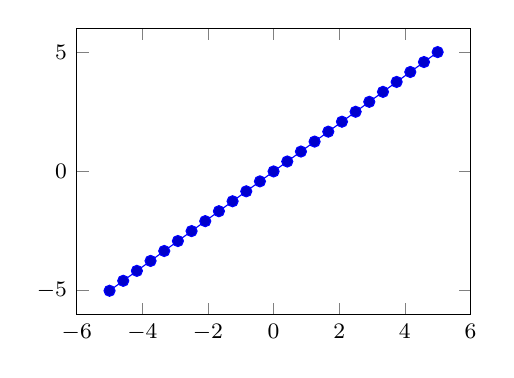
\begin{tikzpicture}
\begin{axis}[
    width=5cm,
    scale only axis,
]
    \addplot {x};
\end{axis}
\end{tikzpicture}
\end{codeexample}

    \paragraph{Note:}

    changing |width| and/or |height| changes \emph{only} the unit vector sizes.
    In particular, it does not change the font size for any axis description,
    nor does it change the default spacing between adjacent tick labels. It is
    best practice to use |width|/|height| for ``small'' changes, i.e.\@ changes
    for which the font size should remain the same. Consider using one of the
    styles |normalsize|, |small|, |footnotesize|, or |tiny| which are described
    in Section~\ref{sec:scaling:styles} on page~\pageref{sec:scaling:styles},
    and \emph{then} change to your desired dimensions if you need a different
    ``quality'' of scaling.

    \begin{command}{\axisdefaultwidth}
        This macro defines the default width. It is preset to |240pt|.

        This default width defines the aspect ratio which will be used whenever
        just one of |width| or |height| is specified: the aspect ratio is the
        ratio between |\axisdefaultwidth| and |\axisdefaultheight|.

        You can change it using
        %
\begin{codeexample}[code only]
\def\axisdefaultwidth{10cm}
\end{codeexample}
    \end{command}
\end{pgfplotskey}

\begin{pgfplotskey}{height=\marg{dimen} (initially empty)}
    Works in the same way as |width| except that an empty value |height={}|
    defaults to ``use either |\axisdefaultheight| or scale proportionally if
    just |width| has been changed''.

    \begin{command}{\axisdefaultheight}
        This macro defines the default height. It is preset to |207pt|.

        See |\axisdefaultwidth|.
    \end{command}
\end{pgfplotskey}

\begin{pgfplotskey}{scale only axis=\mchoice{true,false} (initially false)}
    If |scale only axis| is enabled, |width| and |height| apply only to the
    axis rectangle. Consequently, the resulting figure is larger that |width|
    and |height| (because of any axis descriptions). However, the axis box has
    exactly the prescribed target dimensions.

    If |scale only axis=false| (the default), \PGFPlots{} will try to produce
    the desired width \emph{including} labels, titles and ticks.
\end{pgfplotskey}

\begin{pgfplotsxykeylist}{%
    \x=\marg{dimen} (initially empty),
    \x={\{(\meta{x},\meta{y})\}}%
}
        \index{x!Assign unit vector}%
        \index{y!Assign unit vector}%
        \index{z!Assign unit vector}%
        \index{Unit vector!Assign}%
        \index{3d view!Assign unit vectors}%
        \index{View!Assign unit vectors}%
    Allows to assign zero, one, two, or three of the target unit vectors.

    In this context, a ``unit vector'' is a two-dimensional vector which
    defines the projection onto the canvas: every logical plot coordinate
    $(x,y)$ is drawn at the canvas position
    %
        \begin{equation*}
            x \cdot
                \begin{bmatrix}
                    e_{xx} \\
                    e_{xy}
                \end{bmatrix}
                    + y \cdot
                        \begin{bmatrix}
                            e_{yx} \\
                            e_{yy}
                        \end{bmatrix}.
        \end{equation*}
    %
    The unit vectors $e_x$ and $e_y$ determine the paper position in the
    current (always two dimensional) image. For a standard three-dimensional
    axis, a plot coordinate $(x,y,z)$ is drawn at
    %
        \begin{equation*}
            x \cdot
                \begin{bmatrix}
                    e_{xx} \\
                    e_{xy}
                \end{bmatrix}
                    + y \cdot
                        \begin{bmatrix}
                            e_{yx} \\
                            e_{yy}
                        \end{bmatrix}
                            + z \cdot
                                \begin{bmatrix}
                                    e_{zx} \\
                                    e_{zy}
                                \end{bmatrix}.
        \end{equation*}

    The initial setting assigns empty values to each of these keys, i.e.\@
    |x={},y={},z={}|. In this case, \PGFPlots{} is free to choose these vectors
    as best. To this end, it uses |width|, |height|, |scale mode|,
    |plot box ratio|, |unit vector ratio|, |view|, and the axis limits.

    The key |x=|\marg{dimen} simply sets $e_x = (\meta{dimen},0)^T $ while
    |y=|\marg{dimen} sets $e_y = (0,\meta{dimen})^T$. Using |z=|\marg{dimen}
    results in $e_z = (\meta{dimen},\meta{dimen})^T$. In this context,
    \meta{dimen} is any \TeX{} size like |1mm|, |2cm| or |5pt|. Note that you
    should not use negative values for \meta{dimen} (consider using |x dir| and
    its variants to reverse axis directions).
    %
\begin{codeexample}[]
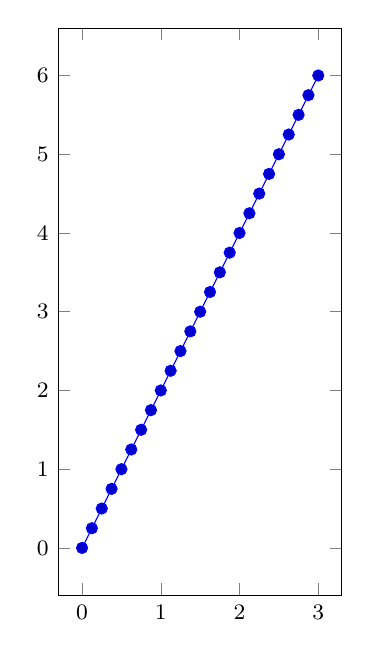
\begin{tikzpicture}
\begin{axis}[
    x=1cm,
    y=1cm,
]
    \addplot expression [domain=0:3] {2*x};
\end{axis}
\end{tikzpicture}
\end{codeexample}

\begin{codeexample}[]
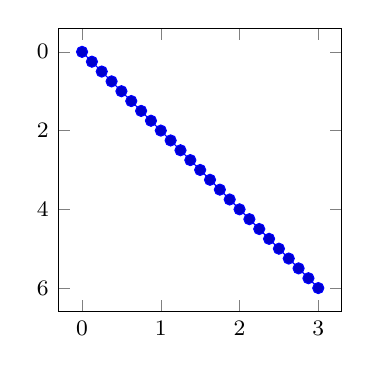
\begin{tikzpicture}
\begin{axis}[
    x=1cm,
    y=0.5cm,
    y dir=reverse,
]
    \addplot expression [domain=0:3] {2*x};
\end{axis}
\end{tikzpicture}
\end{codeexample}

    Note that if you change the unit vector for just one direction, the other
    vector(s) will be chosen by \PGFPlots{} -- and scaled in order to fill the
    prescribed |width| and |height| as best as \PGFPlots{} can (but see remarks
    for three-dimensional plots at the end of this key).
    %
\begin{codeexample}[]
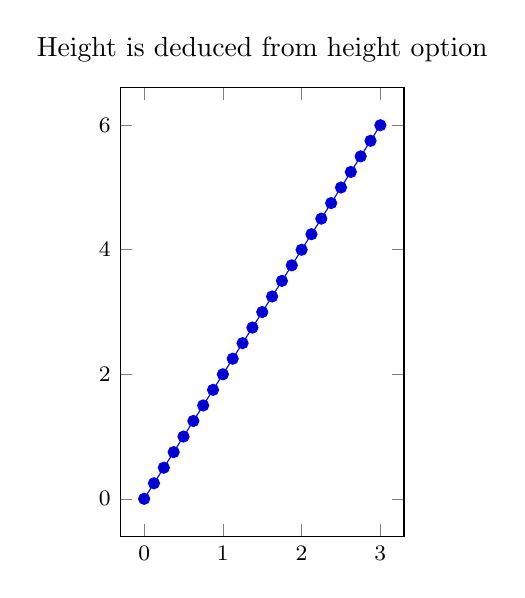
\begin{tikzpicture}
\begin{axis}[
    x=1cm,
    title=Height is deduced from height option,
]
    \addplot expression [domain=0:3] {2*x};
\end{axis}
\end{tikzpicture}
\end{codeexample}

    The second syntax, |x={(|\meta{x}|,|\meta{y}|)}| sets $e_x =
    (\meta{x},\meta{y})^T$ explicitly.\footnote{Please note that you need extra
    curly braces around the vector. Otherwise, the comma will be interpreted as
    separator for the next key--value pair.} The corresponding keys for |y| and
    |z| work in a similar way. This allows to define skewed or rotated axes.

\begin{codeexample}[]
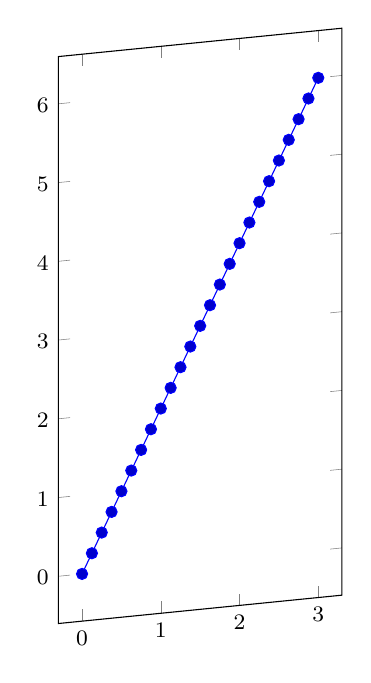
\begin{tikzpicture}
\begin{axis}[
    x={(1cm,0.1cm)},
    y=1cm,
]
    \addplot expression [domain=0:3] {2*x};
\end{axis}
\end{tikzpicture}
\end{codeexample}

\begin{codeexample}[]
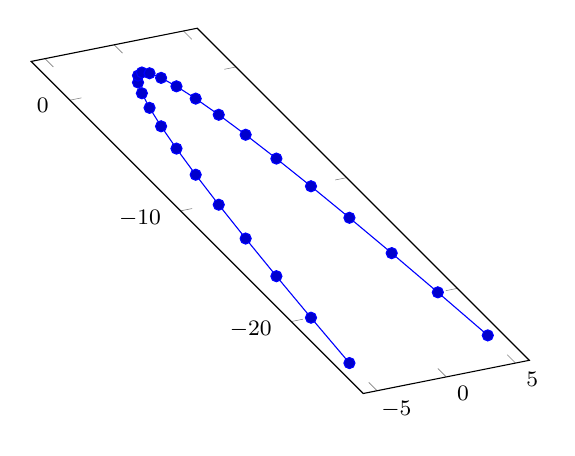
\begin{tikzpicture}
\begin{axis}[
    x={(5pt,1pt)},
    y={(-4pt,4pt)},
]
    \addplot {1-x^2};
\end{axis}
\end{tikzpicture}
\end{codeexample}

    Setting |x| and/or |y| for logarithmic axis will set the dimension used for
    $1 \cdot e \approx 2.71828$ (or whatever has been set as |log basis x|).

    Please note that it is \emph{not} possible to specify |x| as argument to
    |tikzpicture|. The option
    %
\begin{codeexample}[code only]
\begin{tikzpicture}[x=1.5cm]
\begin{axis}
    ...
\end{axis}
\end{tikzpicture}
\end{codeexample}
    %
    does not have any effect because an axis rescales its coordinates (see the
    |width| option).

    Note that providing unit vectors explicitly usually causes \PGFPlots{} to
    ignore any other scaling options. In other words: if you say |y=0.1cm|,
    \PGFPlots{} will use $(0\text{cm},0.1\text{cm})$ as $y$ projection vector.
    However, if you add |scale mode=scale uniformly|, you allow \PGFPlots{} to
    change the \emph{lengths} of your vectors. Of course, it will keep their
    relative directions and relative sizes. In this case, \PGFPlots{} will try
    to determine a good common scaling factor \emph{and} it will try to change
    the axis limits in order to fill the prescribed |width| and |height| (see
    the documentation for |scale mode| for details).
    %
\begin{codeexample}[]
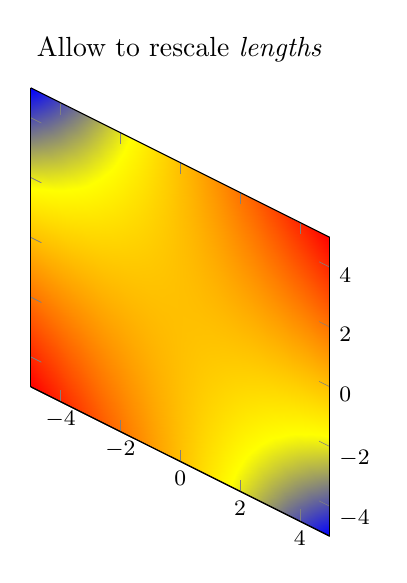
\begin{tikzpicture}
\begin{axis}[
    title=Allow to rescale \emph{lengths},
    x={(0.1cm,-0.05cm)},
    y=0.1cm,
    z=0cm,
    axis on top,
    scale mode=scale uniformly,
]
    \addplot3 [surf,shader=interp] {x*y};
\end{axis}
\end{tikzpicture}
\end{codeexample}
    %
    \noindent In the example above, \PGFPlots{} decided that it should only
    rescale units -- at the expensive of the |width| constraint.


    \paragraph{Changes to font sizes:}

    see also Section~\ref{sec:scaling:styles} if you want to change font sizes
    or the density of tick labels in a simple way.


    \paragraph{Explicit units for 3D axes:}

    As of version~1.5, it is also possible to supply unit vectors to
    three-dimensional axes. In this case, the following extra assumptions need
    to be satisfied:
    %
    \begin{enumerate}
        \item If you want to control three-dimensional units, you need to
            provide \emph{all} of |x|, |y|, and |z| keys. For two-dimensional
            axes, it is also supported to supply just one of |x| or |y|.
        \item Any provided three-dimensional unit vectors are assumed to form
            a \emph{right-handed coordinate system}. In other words: take
            your right hand, let the thumb point into the |x| direction, the
            index finger in |y| direction and the middle finger in |z|
            direction. If that is impossible, the \PGFPlots{} output will be
            wrong. The reason for this assumption is that \PGFPlots{} needs
            to compute the view direction out of the provided units (see
            below).

            Consider using |x dir=reverse| or its variants in case you want
            to reverse directions.
        \item For three-dimensional axes, \PGFPlots{} computes a view
            direction out of the provided unit vectors. The view direction is
            required to allow the |z buffer| feature (i.e.\@ to decide about
            depths).\footnote{\PGFPlots{} provides a debug option called
            \texttt{view dir=\marg{x}\marg{y}\marg{z}} to override the view
            direction, should that ever be interesting.}
    \end{enumerate}
    %
    This feature is used to for the \verbpdfref{\addplot3 graphics} feature,
    compare the examples in Section~\ref{sec:plotgraphics3d} on
    page~\pageref{sec:plotgraphics3d}.


    \paragraph{Limitations:}

    Unfortunately, skewed axes are \textbf{not available for bar plots}.
        \index{Errors!Skewed axes and bar plots}%
        \index{Bar Plots!Skewed axes problems}%
\end{pgfplotsxykeylist}

\begin{pgfplotsxykey}{\x mode=\mchoice{normal,linear,log} (initially normal)}
    Allows to choose between linear (=normal) or logarithmic axis scaling or
    log plots for each $x,y,z$-combination.

    Logarithmic plots use the current setting of |log basis x| and its variants
    to determine the basis (default is $e$).
    % FIXME : replicated in pgfplots.reference.specifyrange.tex
\end{pgfplotsxykey}

{\def\pgfmanualpdflabel#1#2{}
\begin{pgfplotsxykey}{\x\ dir=\mchoice{normal,reverse} (initially normal)}
    Allows to reverse axis directions such that values are given in decreasing
    order.

    This key is documented in all detail on page~\pageref{key:pgfplots:xydir}.
\end{pgfplotsxykey}
}

\begin{pgfplotskey}{axis equal=\marg{true,false} (initially false)}
    Each unit vector is set to the same length while the axis dimensions stay
    constant. Afterwards, the size ratios for each unit in $x$ and $y$ will be
    the same.

    Axis limits will be enlarged to compensate for the scaling effect.
    %
\begin{codeexample}[]
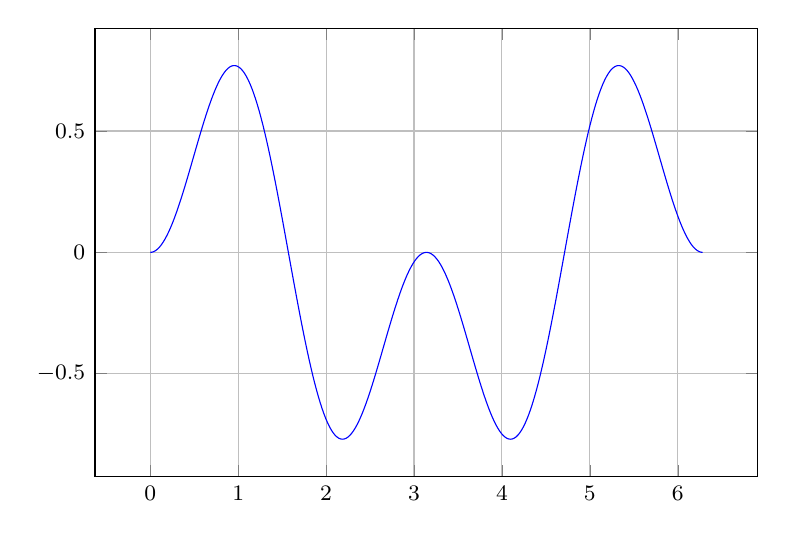
\begin{tikzpicture}
    \begin{axis}[axis equal=false,grid=major]
        \addplot [blue] expression [domain=0:2*pi,samples=300] {sin(deg(x))*sin(2*deg(x))};
    \end{axis}
\end{tikzpicture}
    \hspace{1cm}
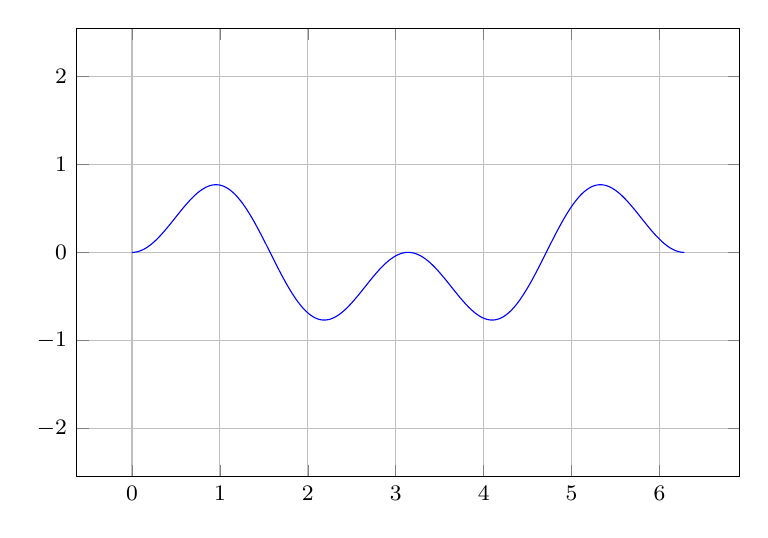
\begin{tikzpicture}
    \begin{axis}[axis equal=true,grid=major]
        \addplot [blue] expression [domain=0:2*pi,samples=300] {sin(deg(x))*sin(2*deg(x))};
    \end{axis}
\end{tikzpicture}
\end{codeexample}

\begin{codeexample}[]
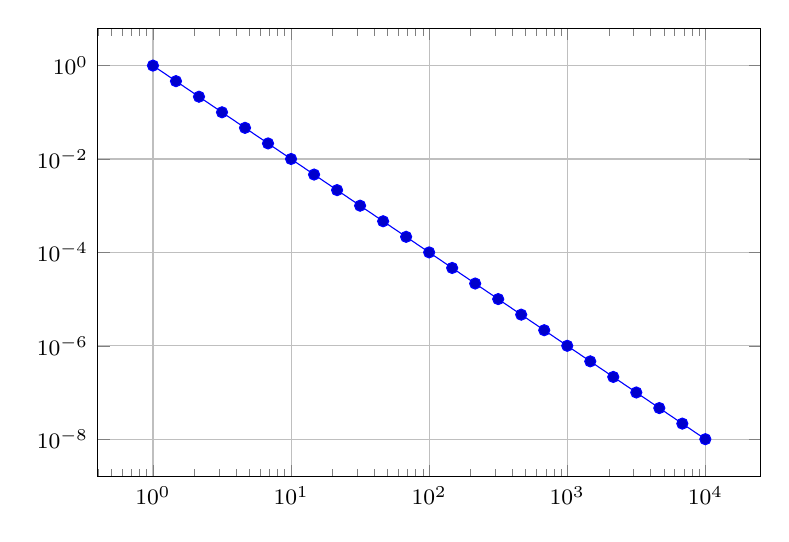
\begin{tikzpicture}
    \begin{loglogaxis}[axis equal=false,grid=major]
        \addplot expression [domain=1:10000] {x^-2};
    \end{loglogaxis}
\end{tikzpicture}
    \hspace{1cm}
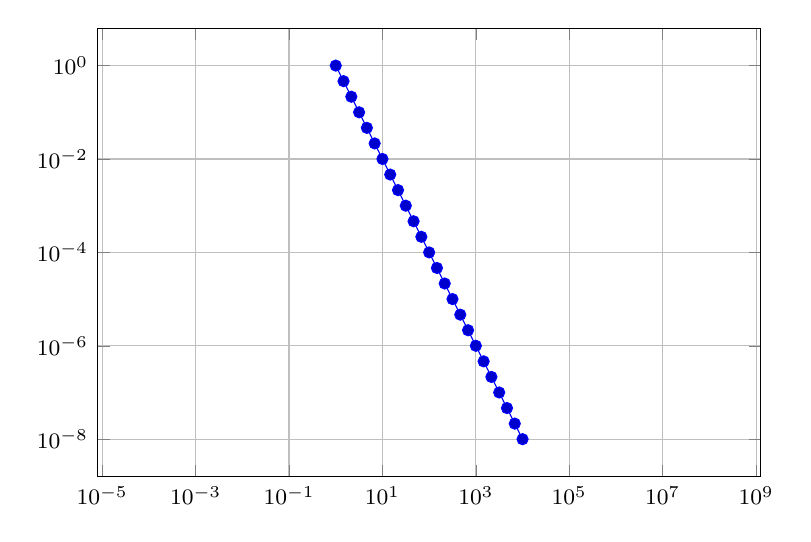
\begin{tikzpicture}
    \begin{loglogaxis}[axis equal=true,grid=major]
        \addplot expression [domain=1:10000] {x^-2};
    \end{loglogaxis}
\end{tikzpicture}
\end{codeexample}

\message{'warning /pgfplots/warning/approx empty range enlarged' is expected here.^^J}%
\begin{codeexample}[]
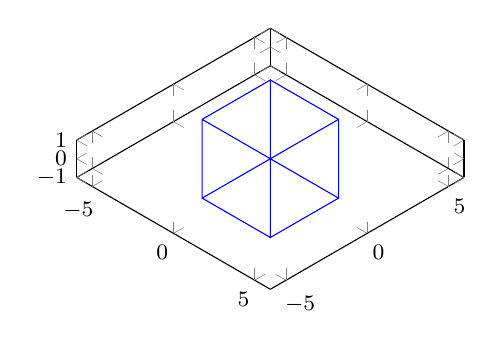
\begin{tikzpicture}
\begin{axis}[axis equal,small,view={45}{35.26}]
    \addplot3 [mark=cube, blue, mark size=1cm]
        coordinates {(0,0,0)};
\end{axis}
\end{tikzpicture}
\end{codeexample}

    The configuration |axis equal=true| is actually just a style which sets
    |unit vector ratio=1 1 1,unit rescale keep size=true|.
\end{pgfplotskey}

\begin{pgfplotskey}{axis equal image=\marg{true,false} (initially false)}
    Similar to |axis equal|, but the axis limits will stay constant as well
    (leading to smaller images).
    %
\begin{codeexample}[]
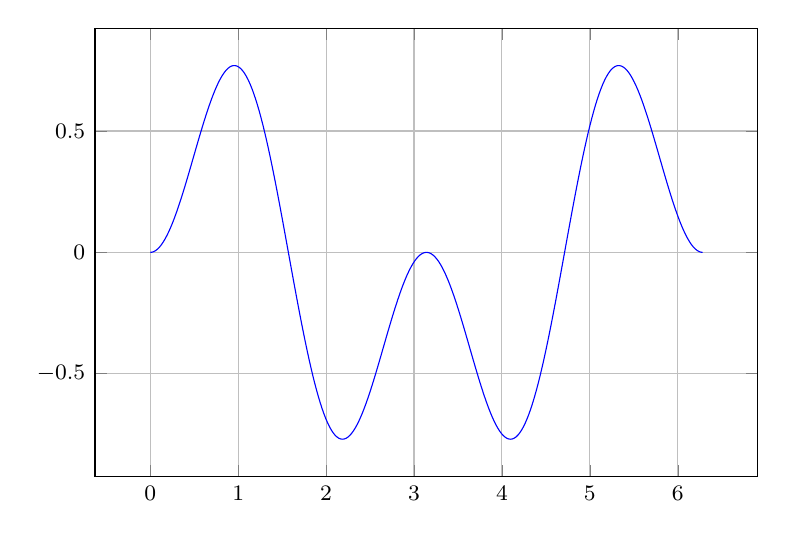
\begin{tikzpicture}
    \begin{axis}[axis equal image=false,grid=major]
        \addplot [blue] expression [domain=0:2*pi,samples=300] {sin(deg(x))*sin(2*deg(x))};
    \end{axis}
\end{tikzpicture}
    \hspace{1cm}
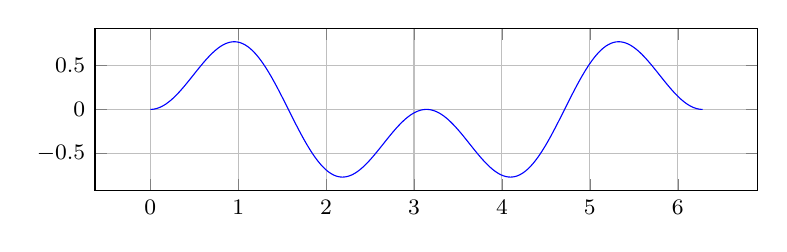
\begin{tikzpicture}
    \begin{axis}[axis equal image=true,grid=major]
        \addplot [blue] expression [domain=0:2*pi,samples=300] {sin(deg(x))*sin(2*deg(x))};
    \end{axis}
\end{tikzpicture}
\end{codeexample}

\begin{codeexample}[]
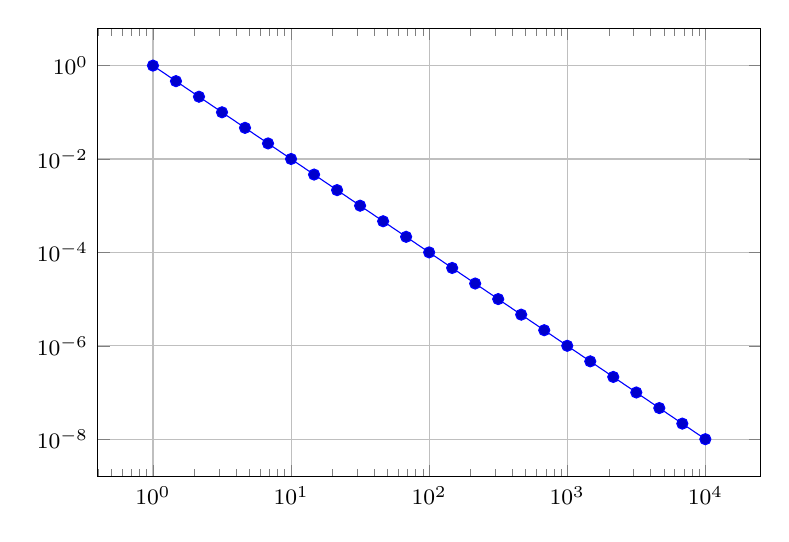
\begin{tikzpicture}
    \begin{loglogaxis}[axis equal image=false,grid=major]
        \addplot expression [domain=1:10000] {x^-2};
    \end{loglogaxis}
\end{tikzpicture}
\hspace{1cm}
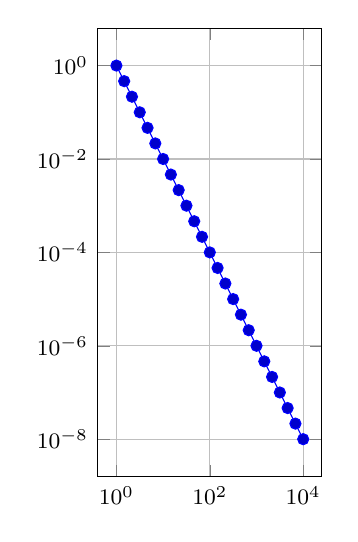
\begin{tikzpicture}
    \begin{loglogaxis}[axis equal image=true,grid=major]
        \addplot expression [domain=1:10000] {x^-2};
    \end{loglogaxis}
\end{tikzpicture}
\end{codeexample}
    %
    The configuration |axis equal image=true| is actually just a style which
    sets |unit vector ratio=1 1 1,unit rescale keep size=false|.
\end{pgfplotskey}

\begin{pgfplotskey}{unit vector ratio=\marg{rx ry rz} (initially empty)}
    Allows to provide custom unit vector ratios.

    The key allows to tell \PGFPlots{} that, for example, one unit in $x$
    direction should be twice as long as one unit in $y$ direction:
    %
\begin{codeexample}[]
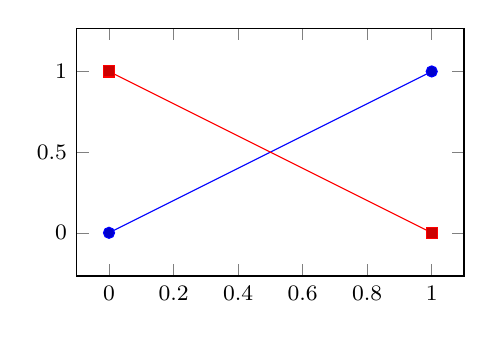
\begin{tikzpicture}
\begin{axis}[unit vector ratio=2 1,small]
    \addplot coordinates {(0,0) (1,1)};
    \addplot table [row sep=\\,col sep=&] {
        x & y \\
        0 & 1 \\
        1 & 0 \\
    };
\end{axis}
\end{tikzpicture}
\end{codeexample}
    %
    \noindent Providing |unit vector ratio=2 1| means that
    $\frac{||e_x||}{||e_y||} = 2$ where each coordinate $(x,y)$ is placed at $x
    e_x + y e_y \in \R^2$ (see the documentation for |x| and |y| options). Note
    that |axis equal| is nothing but |unit vector ratio=1 1 1|.

    The arguments \meta{rx}, \meta{ry}, and \meta{rz} are ratios for $x$, $y$
    and $z$ vectors, respectively. For two-dimensional axes, only \meta{rx} and
    \meta{ry} are considered; they are provided relative to the $y$-axis. In
    other words: the $x$ unit vector will be \meta{rx}$/$\meta{ry} times
    longer than the $y$ unit vector. For three-dimensional axes, all three
    arguments can be provided; they are interpreted relative to the $z$ unit
    vector. Thus, a three dimensional axis with |unit vector ratio=1 2 4| will
    have an $x$ unit which is $\nicefrac 14$ the length of the $z$ unit, and a
    $y$ unit which is $\nicefrac24$ the length of the $z$ unit.

    Trailing values of |1| can be omitted, i.e.\@ |unit vector ratio=2 1| is
    the same as |unit vector ratio=2|; and |unit vector ratio=3 2 1| is the
    same as |unit vector ratio=3 2|. An empty value |unit vector ratio={}|
    disables unit vector rescaling.

    Note that an active |unit vector ratio| will implicitly set
    |scale mode=scale uniformly|.\footnote{This has been introduced in version
    1.6. For older versions, the axis equal feature produced wrong results for
    three-dimensional axes.}

    \begin{pgfplotskeylist}{%
        unit vector ratio*=\marg{rx ry rz},
        unit rescale keep size=\mchoice{%
                true,
                false,
                unless limits declared%
            } (initially unless limits declared)%
    }
    \label{key:unit:rescale:keep:size}
        In the default configuration, \PGFPlots{} maintains the original axis
        dimensions even though |unit vector ratio| involves different scalings.

        It does so by enlarging the limits.
        %
\begin{codeexample}[]
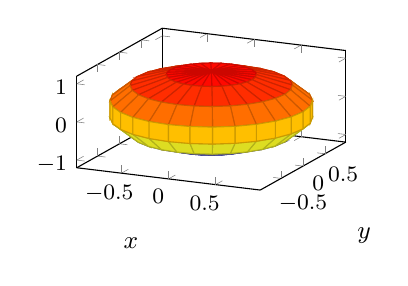
\begin{tikzpicture}
    \begin{axis}[footnotesize,xlabel=$x$,ylabel=$y$,unit vector ratio=]
        \addplot3 [surf,z buffer=sort,samples=15,
            variable=\u, variable y=\v,
            domain=0:180, y domain=0:360]
               ({cos(u)*sin(v)}, {sin(u)*sin(v)}, {cos(v)});
    \end{axis}
\end{tikzpicture}
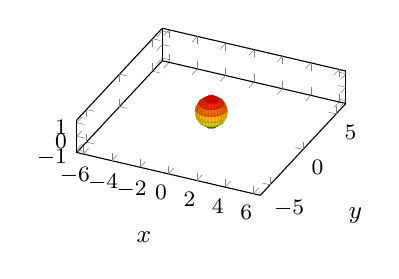
\begin{tikzpicture}
    \begin{axis}[footnotesize,xlabel=$x$,ylabel=$y$,unit vector ratio=1 1 1]
        \addplot3 [surf,z buffer=sort,samples=15,
            variable=\u, variable y=\v,
            domain=0:180, y domain=0:360]
               ({cos(u)*sin(v)}, {sin(u)*sin(v)}, {cos(v)});
    \end{axis}
\end{tikzpicture}
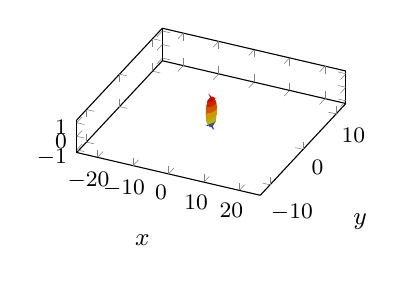
\begin{tikzpicture}
    \begin{axis}[footnotesize,xlabel=$x$,ylabel=$y$,unit vector ratio=0.25 0.5]
        \addplot3 [surf,z buffer=sort,samples=15,
            variable=\u, variable y=\v,
            domain=0:180, y domain=0:360]
               ({cos(u)*sin(v)}, {sin(u)*sin(v)}, {cos(v)});
    \end{axis}
\end{tikzpicture}
\end{codeexample}
        %
        \noindent The example above has the same plot, with three different
        unit ratios. The first has no limitations (it is the default
        configuration). The second uses the same length for each unit vector
        and enlarges the limits in order to maintain the same dimensions. The
        third example has an $x$ unit which is $\nicefrac14$ the length of a
        $z$ unit, and an $y$~unit which is $\nicefrac12$ the length of a
        $z$~unit.

        \PGFPlots{} does its best to respect the involved scaling options (the
        prescribed |width| and |height|, the |unit vector ratio|, and any
        specified axis limits). In the case above, it enlarged the horizontal
        limits and kept the $z$~limit as is. See |scale mode| and its
        documentation for details about the involved algorithm and its
        parameters.

        The |unit rescale keep size=false| key, or, equivalently,
        |unit vector ratio*=...|, does not enlarge limits:
        %
\begin{codeexample}[]
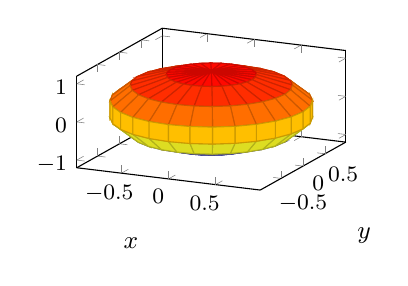
\begin{tikzpicture}
    \begin{axis}[footnotesize,xlabel=$x$,ylabel=$y$,unit vector ratio=]
        \addplot3 [surf,z buffer=sort,samples=15,
            variable=\u, variable y=\v,
            domain=0:180, y domain=0:360]
               ({cos(u)*sin(v)}, {sin(u)*sin(v)}, {cos(v)});
    \end{axis}
\end{tikzpicture}
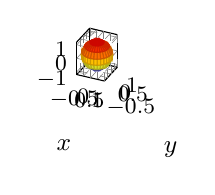
\begin{tikzpicture}
    \begin{axis}[footnotesize,xlabel=$x$,ylabel=$y$,
        unit rescale keep size=false,
        unit vector ratio=1 1 1]
        \addplot3 [surf,z buffer=sort,samples=15,
            variable=\u, variable y=\v,
            domain=0:180, y domain=0:360]
               ({cos(u)*sin(v)}, {sin(u)*sin(v)}, {cos(v)});
    \end{axis}
\end{tikzpicture}
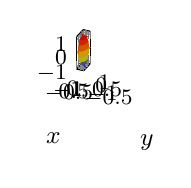
\begin{tikzpicture}
    \begin{axis}[footnotesize,xlabel=$x$,ylabel=$y$,
        unit vector ratio*=0.25 0.5, % the '*' implies 'unit rescale keep size=false'
    ]
        \addplot3 [surf,z buffer=sort,samples=15,
            variable=\u, variable y=\v,
            domain=0:180, y domain=0:360]
               ({cos(u)*sin(v)}, {sin(u)*sin(v)}, {cos(v)});
    \end{axis}
\end{tikzpicture}
\end{codeexample}
        %
        The key |unit rescale keep size| also affects
        |scale mode=scale uniformly| (which is closely related to
        |axis equal|).

        Here is the reference of the value of |unit rescale keep size|: the
        value \declaretext{true} means that \PGFPlots{} will enlarge limits in
        order to keep the size. It will try to respect user provided limits,
        but if the user provided \emph{all} limits, it will \emph{override} the
        user-provided limits and will rescale them. Thus, |true| gives higher
        priority to the axis size than to user-provided limits. The choice
        \declaretext{false} will never rescale axis limits. The choice
        \declaretext{unless limits declared} is a mixture: it will enlarge
        limits unless the user provided them. If the user provides all limits
        explicitly, this choice is the same as |false|.
    \end{pgfplotskeylist}
\end{pgfplotskey}

\begin{pgfplotsxykeylist}{%
    \x\ post scale=\marg{scale} (initially empty),
    scale=\marg{scale} (initially empty)%
}
    Lets \PGFPlots{} compute the axis scaling based on |width|, |height|,
    |view|, |plot box ratio|, |axis equal| or explicit unit vectors with |x|,
    |y|, |z| and \emph{rescales} the resulting vector(s) according to
    \meta{scale}.

    The |scale| key sets all three keys to the same \meta{uniform scale} value.
    This is effectively the same as if you rescale the complete axis (without
    changing sizes of descriptions).

    The other keys allow individually rescaled axes.
    %
\begin{codeexample}[]
\begin{tikzpicture}
    \begin{axis}[y post scale=1]
        \addplot {x};
    \end{axis}
\end{tikzpicture}
\begin{tikzpicture}
    \begin{axis}[y post scale=2]
        \addplot {x};
    \end{axis}
\end{tikzpicture}
\end{codeexample}
    %
    Thus, the axis becomes \emph{larger}. This overrules any previous scaling.

\begin{codeexample}[]
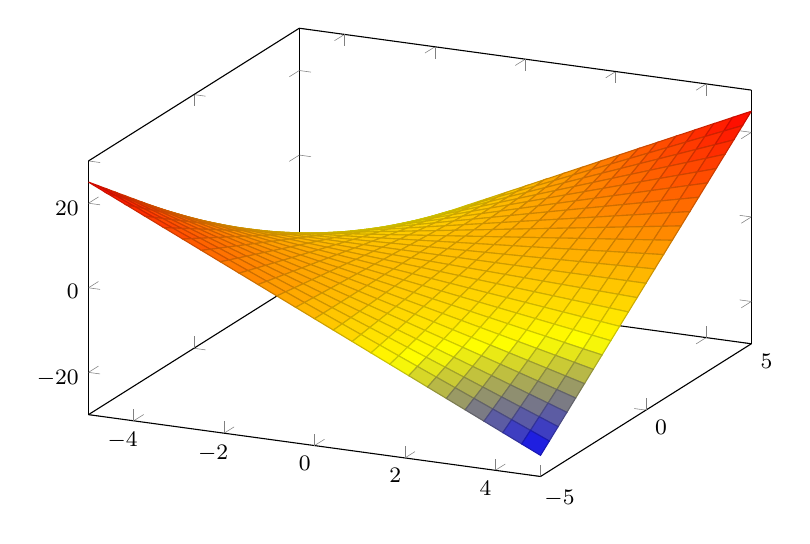
\begin{tikzpicture}
    \begin{axis}[z post scale=1]
        \addplot3 [surf] {x*y};
    \end{axis}
\end{tikzpicture}
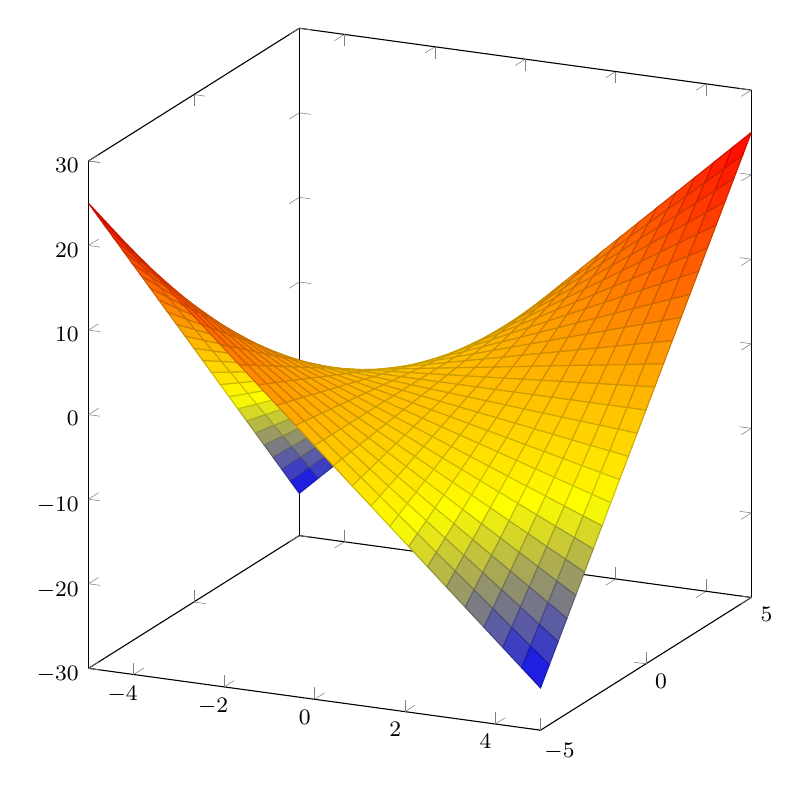
\begin{tikzpicture}
    \begin{axis}[z post scale=2]
        \addplot3 [surf] {x*y};
    \end{axis}
\end{tikzpicture}
\end{codeexample}
\end{pgfplotsxykeylist}


\subsection{Scaling Descriptions: Predefined Styles}
\label{sec:scaling:styles}

It is reasonable to change font sizes, marker sizes etc.\@ together with the
overall plot size: Large plots should also have larger fonts and small plots
should have small fonts and a smaller distance between ticks.

\begin{keylist}{%
    /tikz/font=\mchoice{%
        \textbackslash normalfont,
        \textbackslash small,
        \textbackslash tiny,
        $\dotsc$%
    },
    /pgfplots/max space between ticks=\marg{integer},
    /pgfplots/try min ticks=\marg{integer},
    /tikz/mark size=\marg{integer}%
}
    These keys should be adjusted to the figure's dimensions. Use
    %
\begin{codeexample}[code only]
\pgfplotsset{
    tick label style={font=\footnotesize},
    label style={font=\small},
    legend style={font=\small},
}
\end{codeexample}
    %
    to provide different fonts for different descriptions.

    The keys |max space between ticks| and |try min ticks| are described on
    page~\pageref{maxspacebetweenticks} and configure the approximate distance
    and number of successive tick labels (in |pt|). Please omit the |pt| suffix
    here.
\end{keylist}

There are a couple of predefined scaling styles which set some of these
options:

\begin{stylekey}{/pgfplots/normalsize}
    Reinitializes the standard scaling options of \PGFPlots{}.
    %
\begin{codeexample}[]
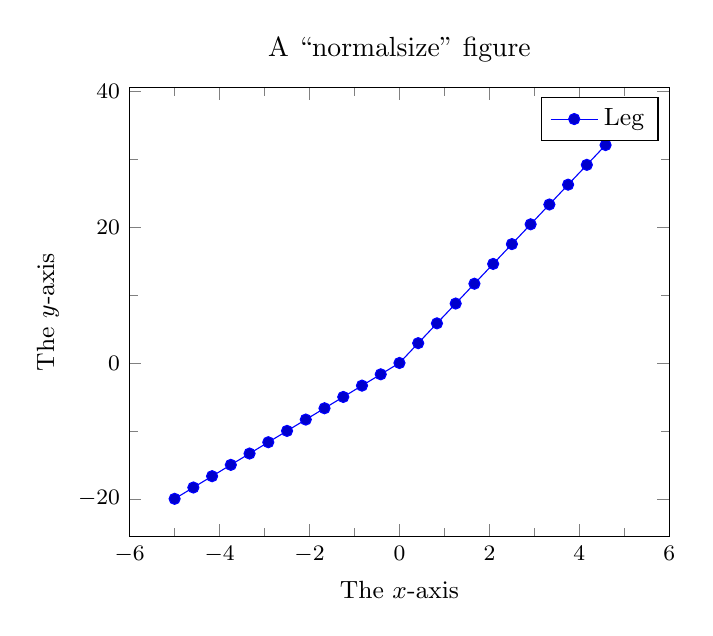
\begin{tikzpicture}
    \begin{axis}[normalsize,
        title=A ``normalsize'' figure,
        xlabel=The $x$-axis,
        ylabel=The $y$-axis,
        minor tick num=1,
        legend entries={Leg},
    ]
        \addplot {max(4*x,7*x)};
    \end{axis}
\end{tikzpicture}
\end{codeexample}

    The initial setting is
\begin{codeexample}[code only]
\pgfplotsset{
    normalsize/.style={
        /pgfplots/width=240pt,
        /pgfplots/height=207pt,
        /pgfplots/max space between ticks=35,
    },
}
\end{codeexample}
\end{stylekey}

\begin{stylekey}{/pgfplots/small}
    Redefines several keys such that the axis is ``smaller''.
    %
\begin{codeexample}[]
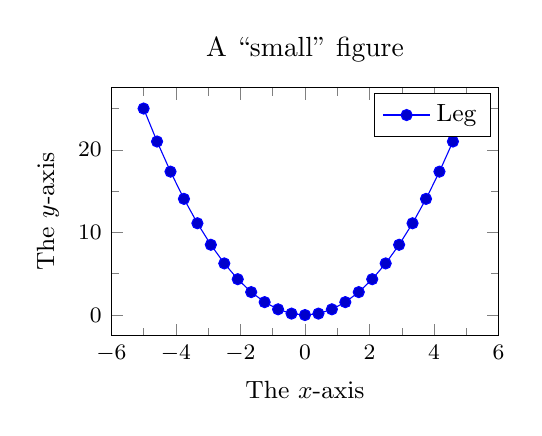
\begin{tikzpicture}
\begin{axis}[
    small,
    title=A ``small'' figure,
    xlabel=The $x$-axis,
    ylabel=The $y$-axis,
    minor tick num=1,
    legend entries={Leg},
]
    \addplot {x^2};
\end{axis}
\end{tikzpicture}
\end{codeexample}
    %
    The initial setting is
    %
\begin{codeexample}[code only]
\pgfplotsset{
    small/.style={
        width=6.5cm,
        height=,
        tick label style={font=\footnotesize},
        label style={font=\small},
        max space between ticks=25,
    },
}
\end{codeexample}
    %
    Feel free to redefine the scaling -- the option may still be useful to get
    more ticks without typing too much. You could, for example, set
    |small,width=6cm|.
\end{stylekey}

\begin{stylekey}{/pgfplots/footnotesize}
    Redefines several keys such that the axis is even smaller. The tick labels
    will have |\footnotesize|.
    %
\begin{codeexample}[]
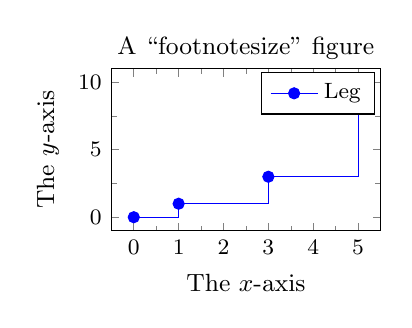
\begin{tikzpicture}
\begin{axis}[
    footnotesize,
    title=A ``footnotesize'' figure,
    xlabel=The $x$-axis,
    ylabel=The $y$-axis,
    minor tick num=1,
    legend entries={Leg},
]
    \addplot+ [const plot] coordinates {
        (0,0) (1,1) (3,3) (5,10)
    };
\end{axis}
\end{tikzpicture}
\end{codeexample}
    %
    The initial setting is
    %
\begin{codeexample}[code only]
\pgfplotsset{
    footnotesize/.style={
        width=5cm,
        height=,
        legend style={font=\footnotesize},
        tick label style={font=\footnotesize},
        label style={font=\small},
        title style={font=\small},
        every axis title shift=0pt,
        max space between ticks=15,
        every mark/.append style={mark size=8},
        major tick length=0.1cm,
        minor tick length=0.066cm,
    },
}
\end{codeexample}
    %
    As for |small|, it can be convenient to set |footnotesize| and set |width|
    afterwards.

    You will need |compat=1.3| or newer for this to work.
\end{stylekey}

\begin{stylekey}{/pgfplots/tiny}
    Redefines several keys such that the axis is very small. Most descriptions
    will have |\tiny| as fontsize.
    %
\begin{codeexample}[]
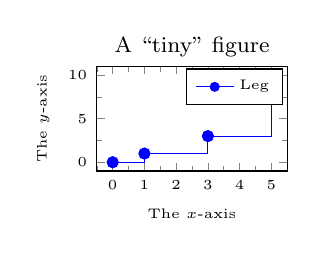
\begin{tikzpicture}
\begin{axis}[tiny,
    title=A ``tiny'' figure,
    xlabel=The $x$-axis,
    ylabel=The $y$-axis,
    minor tick num=1,
    legend entries={Leg},
]
    \addplot+ [const plot] coordinates {
        (0,0) (1,1) (3,3) (5,10)
    };
\end{axis}
\end{tikzpicture}
\end{codeexample}
    %
    The initial setting is
    %
\begin{codeexample}[code only]
\pgfplotsset{
    tiny/.style={
        width=4cm,
        height=,
        legend style={font=\tiny},
        tick label style={font=\tiny},
        label style={font=\tiny},
        title style={font=\footnotesize},
        every axis title shift=0pt,
        max space between ticks=12,
        every mark/.append style={mark size=6},
        major tick length=0.1cm,
        minor tick length=0.066cm,
        every legend image post/.append style={scale=0.8},
    },
}
\end{codeexample}
    %
    As for |small|, it can be convenient to use |tiny,width=4.5cm| to adjust
    the width.

    You will need |compat=1.3| or newer for this to work.
\end{stylekey}


\subsection{Scaling Strategies}

The content of this section is quite involved -- and its knowledge is typically
unnecessary because by default, \PGFPlots{} controls the involved stuff
automatically. You may want to skip this section.

\begin{pgfplotskey}{scale mode=\mchoice{auto,none,stretch to fill,scale uniformly} (initially auto)}
    Specifies how to choose the (individual) unit vector scaling factors, their
    length ratios, and perhaps the axis limits in order to fill the prescribed
    |width| and |height|.

    The |scale mode| implementation expects some ``initial'' set of unit
    vectors. This initial set of unit vectors is determined as follows: for
    standard two-dimensional axes, it is simply the unit cube
    $e_x=(1\text{pt},0\text{pt})^T$, $e_y=(0\text{pt},1\text{pt})^T$, $e_z=0$.
    For three-dimensional axes, it is the outcome of the two keys |view| and
    |plot box ratio|. If you provided units explicitly by means of one of |x|,
    |y|, or |z|, this value is the initial unit vector.

    In addition, it expects ``initial'' axis limits (i.e.\@ values of |xmin|,
    |xmax|, etc.). The initial axis limits are those limits which have been
    deduced from your data or which have been provided explicitly. Furthermore,
    the initial axis limits already include changes of the |enlargelimits| key.

    Given the initial set of unit vectors and the initial axis limits, the
    |scale mode| implementation is a kind of ``post-processor'' which creates
    modified unit vectors and modified axis limits in order to satisfy all
    specified constraints. These constraints are |width|, |height|, and
    |unit vector ratio|.

    The initial choice \declaretext{auto} tells \PGFPlots{} to take full
    control over this key. It chooses one of the other possible choices
    depending on the actual context. The choice |auto| evaluates to
    |scale uniformly| if |unit vector ratio| is set. Otherwise it evaluates to
    |stretch to fill|.

    The choice \declaretext{none} does not apply any rescaling at all. Use this
    if prescribed lengths of |x|, |y| (and perhaps |z|) should be used. In
    other words: it ignores |width| and |height|. In this case, you may want to
    set |x post scale| and its variants to rescale units manually. See also
    |disabledatascaling|.

    The choice \declaretext{stretch to fill} takes the initial unit vectors and
    rescales the unit vectors with two \emph{separate} scales: one which
    results in the proper |width| and one which results in the proper |height|.
    As a consequence, the unit vectors are modified and distorted such that the
    final image fits into the prescribed dimensions. This is usually what one
    expects unless one provides unit directions explicitly. This mode does not
    change axis limits. Note that if one of the unit vectors has been provided
    explicitly, \PGFPlots{} will not change it. It will only change the
    remaining axis limits. This mode contradicts |axis equal| or
    |unit vector ratio|.

    The choice \declaretext{scale uniformly} takes the initial unit vectors and
    applies only \emph{one} scaling factor to all units. In this case, there is
    just \emph{one} common scaling factor for both |width| and |height|.
    Naturally, this will result in unsatisfactory results because either the
    final width or the final height will not be met. Therefore, this choice
    will adjust axis limits to get the desired dimensions. Thus, the unit
    vectors have exactly the same size \emph{relations and angles} as they had
    before the scaling; only their magnitude is changed uniformly. In addition,
    axis limits may be changed (with individual scaling factors for each axis
    limit). Note that if unit vectors have been provided explicitly,
    \PGFPlots{} can still rescale it with this choice -- it will keep the
    relative directions and size ratios. The choice |scale uniformly| tries its
    best to modify the degrees of freedom in a ``useful'' way. The precise
    meaning of ``useful'' is the |scale uniformly strategy| key.

    \begin{pgfplotskey}{scale uniformly strategy=\mchoice{%
            auto,
            units only,
            change vertical limits,\\
            change horizontal limits%
        } (initially auto)%
    }
        The |scale uniformly| method requires to determine one \emph{common}
        scaling factor which rescales every axis \emph{unit}. In addition, it
        allows one scaling factor \emph{for each axis limit}, i.e.\@ up to
        three.

        The constraints for this search are that we want to satisfy the
        |width|/|height| constraint, have as few rescaling as possible and that
        we do not want to reduce limits (as this could possibly hide data
        points).

        The choice \declaretext{auto} chooses one of the other possibilities
        automatically. Depending on whether we have two dimensions or three
        dimensions, it compares the available methods and chooses the one which
        does not reduce limits and which involves the fewest rescaling (i.e.\@
        it may compare the outcome of the other strategies). This is the
        default. If you keep the choice |auto|, you do not have to worry about
        the remaining choices. Note that manually provided axis limits will not
        be modified.

        The choice \declaretext{units only} will not enlarge axis limits. It
        will only rescale the units. To this end, it chooses the scaling factor
        such that the \emph{smaller} target dimension is filled as desired. In
        other words: if |width| $<$ |height|, it will scale to satisfy the
        |width| constraint. The |height| constraint will be ignored. The case
        $>$ will be done the other way round. The choice |units only| typically
        results in a square axis as it takes the initial set of unit vectors
        (which are typically the unit box) and scales them with a common
        scaling factor. Consequently, you can choose |units only| if you want a
        boxed axis. You can still change axis limits manually, however.

        The choice \declaretext{change vertical limits} chooses a common
        scaling factor for the unit vectors on order to satisfy the |width| (!)
        constraint. This common scaling factor is similar to |units only| --
        but |units only| can also decide to satisfy the |height| constraint
        whereas |change vertical limits| will scale unit vectors to satisfy
        |width|. In order to satisfy the |height| constraint,
        |change vertical limits| modifies just the vertical limits. For
        two-dimensional axes, this is |ymin| and |ymax|. For three-dimensional
        axes, this is |zmin| and |zmax|. Clearly, there is a chance that it
        will \emph{decrease} the displayed range -- in this case, parts of the
        image will be clipped away. This method \emph{assumes} that the
        vertical axis has not been rotated (i.e.\@ that $e_{yx}=0$ or
        $e_{zx}=0$, respectively). It refuses to work and falls back to
        |units only| for rotates axes. Choose |change vertical limits| if you
        want the image (i.e.\@ the actual content) as wide as possible. You can
        modify |width| and |height| to improve its outcome. Note that manually
        specified axis limits will not be changed, see below for details.

        The choice \declaretext{change horizontal limits} attempts a similar
        approach, but for the horizontal limits: it determines one suitable
        scaling factor which is applied to all unit vectors and modifies
        horizontal axis limits to satisfy the remaining constraints. For
        two-dimensional axes, this is quite simple because we typically have
        $e_{xy} = 0$ (i.e.\@ the $x$ unit vector has vanishing $y$ component)
        and $e_{yx}=0$ such that \PGFPlots{} can change axis limits easily. If
        a two-dimensional axis has an $x$ unit with $e_{xy} \neq 0$, the method
        is not applicable and falls back to |units only|. For three-dimensional
        axes, it assumes that the $z$ vector is not rotated, i.e.\@ $e_{zy} =
        0$ and tries to change limits for both $x$ and $y$. This choice is much
        more involved because here, $x$ and $y$ components are coupled.
        Consequently, the common unit scaling factor and the two involved axis
        limit compensation factors for $x$ and $y$ are tightly coupled as well.
        \PGFPlots{} solves a system of nonlinear equations iteratively to
        arrive at a suitable solution for all three scalings. Use this method
        if |change vertical limits| would clip away parts of the image (because
        it reduced the displayed range) and you do not want to change |width|
        and |height|. The choice |change horizontal limits| will typically
        result in more empty space in the resulting figure. But it will not
        clip away content. Manually specified axis limits will not be changed,
        see below for details.
    \end{pgfplotskey}


    \paragraph{Manually provided axis limits:}

    Any manually provided arguments for |xmin| and its variants are considered
    to be immutable; \PGFPlots{} will not change them. If you assign |xmin|,
    \PGFPlots{} will only change |xmax| and vice versa. If you assign both
    |xmin| and |xmax|, \PGFPlots{} will not change $x$~limits at all. Note that
    if you assign both |xmin| and |xmax|, \PGFPlots{} will simply skip the
    scaling and will give up on the constraints. It will not try to compensate
    the lack of scaling opportunities by changing $y$~limits, for example. This
    has the positive effect that assigning limits does not change the complete
    appearance of your axis. The allowed set of changes to axis limits can be
    configured with the following key.


    \paragraph{Interaction with }|enlargelimits|:

    Note that |enlargelimits| and |scale mode| are independent of another: the
    outcome of |enlargelimits| is used as ``initial axis limits'' and these
    limits may be changed by |scale mode| (even if you said
    |enlargelimits=false|). See the documentation of |enlargelimits| for
    details on this interaction.

    \begin{pgfplotskey}{unit rescale keep size=\mchoice{%
            true,
            false,
            unless limits declared%
        } (initially unless limits declared)%
    }
        In the default configuration \declaretext{unless limits declared}, unit
        rescaling may cause changes to the axis limits in order to keep the
        figure's size intact. However, only those limits which have not been
        declared manually are subject to rescaling: if you say |xmin=1|, only
        |xmax| and the limits for $y$ and $z$ are free to change.

        Setting |unit rescale keep size=|\declaretext{false} will
        \emph{disable} the modification of axis limits altogether, i.e.\@ axis
        limits will not be rescaled to compensate scalings on unit vectors.

        Setting |unit rescale keep size=|\declaretext{true} will always rescale
        limits, even if they have been declared manually.

        This key mainly affects |scale mode=scale uniformly|. This, in turn, is
        used for |axis equal| and |\addplot3 graphics|.

        See also the addition documentation for this key and related examples
        on page~\pageref{key:unit:rescale:keep:size}.
    \end{pgfplotskey}

    The |scale uniformly| choice is implicitly used for |axis equal| and for
    the \verbpdfref{\addplot3 graphics} feature, see the documentation in
    Section~\ref{sec:plotgraphics3d} on page~\pageref{sec:plotgraphics3d} for
    its examples. Note that the common case is that the initial unit vectors
    form the unit cube (i.e.\@ those before scaling, see above). In this case,
    |scale uniformly| is the same as |axis equal|.
\end{pgfplotskey}
